\subsection{Metodo e formalismo di specifica}
L'architettura del progetto verrà esposta seguendo il metodo top-down, si partirà, cioè, dal livello più generale per poi scendere nel dettaglio. I diagrammi di classe, attività e sequenza saranno conformi al formalismo UML 2.x, come previsto nelle Norme di Progetto v1.0.0.

\subsection{Architettura generale}
L'architettura del prodotto che vogliamo realizzare segue il pattern three-tier, che prevede la suddivisione dell'applicazione in tre diversi strati. I tre strati sono dedicati rispettivamente all'interfaccia utente, alla logica funzionale e alla gestione dei dati persistenti e comunicano tra loro secondo le linee generali del modello client-server. L'architettura three-tier permette una maggiore scalabilità e manutenibilità dell'applicazione in quanto è possibile modificare o sostituire uno strato indipendentemente dagli altri.

Attraverso la seguente figura presenteremo i tier dell'architettura adattati al nostro progetto, che saranno approfonditi nel dettaglio nelle sezioni successive del documento.

\begin{figure}[h]
	\centering
	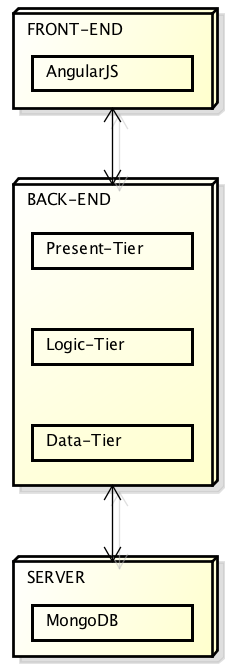
\includegraphics[height=0.6\textheight]{img/architettura_generale}
	\caption[Architettura generale del sistema]{Architettura generale del sistema}
\end{figure}

\textbf{Presentation-Tier}: contiene il front-end dell'applicazione, che si occupa della presentazione dei dati all'utente. Funge da interfaccia tra l'utente e il back-end, interagendo con il tier sottostante.

\textbf{Logic-Tier}: comunica con il livello superiore elaborando le richieste generate da esso e recuperando i dati dal livello inferiore. Questo strato è a sua volta organizzato con un'architettura three-tier per la gestione del back-end dell'applicazione.

\textbf{Data-tier}: questo livello è costituito dal database dell'applicazione ed è dove vengono memorizzate e recuperate le informazioni. Nel nostro caso il database è di tipo non relazionale.

\subsection{Interfaccia REST-like}
Si é scelto di utilizzare uno stile REST-like per quanto riguarda l'interfaccia della componente back-end dell'applicativo \PROGETTO, cioè basato sullo stile REST ma modificato per permettere l'autenticazione e l'utilizzo di determinate operazioni. Più precisamente il comportamento dell'interfaccia con cui si accede agli elementi della collection può considerarsi REST all'interno di una sessione utente, ovvero dall'operazione di login fino a quella di logout. Le motivazioni di tale scelta sono le seguenti:
\begin{itemize}
	\item Semplicità di utilizzo;
	\item Semplicità di integrazione con i framework esistenti (Angular.js);
	\item Indipendenza dal linguaggio di programmazione utilizzato.
	\end{itemize}
	REST utilizza un aggregato di dati con un nome (URI) e una rappresentazione su cui é possibile invocare operazioni CRUD tramite la seguente configurazione:
	
	\begin{table}[h]
		\begin{tabular}{|p{0.2\textwidth}|p{0.35\textwidth}|p{0.35\textwidth}|}
			\toprule
			
			\textbf{Risorsa} & \textbf{URI della collection} \smallbreak
			es. http://site.com/users  & \textbf{URI di un utente} \smallbreak
			es. http:/site.com/users/\{id\} \\
			
			\midrule
			\textbf{GET} & Fornisce informazioni sui membri della collection. & Fornisce una rappresentazione dell'elemento della collection indicato. \\ \midrule
			\textbf{PUT} & Non utilizzata. & Sostituisce l'elemento della collection indicato. Se non esiste lo crea. \\  \midrule
			\textbf{POST} & Crea un nuovo elemento nella collection. La URI del nuovo elemento é generata in automatico e solitamente viene restituita dall'operazione. & Non utilizzata. \\ \midrule
			\textbf{DELETE} & Non utilizzata. & Cancella l'elemento della collection indicato.  \\ \midrule
			
			
			\end{tabular}\\
			\caption{Tabella configurazioni REST}
			
			\end{table}
			
Si é deciso di scegliere il formato JSON come formato di rappresentazione dei dati poiché si integra perfettamente con i framework utilizzati e con il linguaggio Javascript.